%
% Copyright (c) 2013-2023 Aleksey Fedoseev <aleksey@fedoseev.net>
% Copyright (c) 2013-2015 Nikolay Safronov <bfishh@gmail.com>
%
% Permission is granted to copy, distribute and/or modify this document
% under the terms of the GNU Free Documentation License, Version 1.3
% or any later version published by the Free Software Foundation;
% with no Invariant Sections, no Front-Cover Texts, and no Back-Cover Texts.
% A copy of the license is located here: http://www.gnu.org/copyleft/fdl.html.
%

\documentclass[12pt,a4paper]{article}
\usepackage[T2A]{fontenc}
\usepackage{ucs}
\usepackage[utf8]{inputenc}
\usepackage[english]{babel}
\usepackage{indentfirst}
\usepackage{amsmath}
\usepackage{amssymb}
\usepackage{graphicx}
\usepackage{hyperref}
\usepackage{array}
\usepackage{titlesec}
\usepackage{subcaption}
\usepackage{wasysym}
\usepackage{longtable}

\pagestyle{plain}
\parindent=1.25cm
\textheight=24cm
\textwidth=16cm
\topmargin=-1cm
\frenchspacing
\renewcommand{\theequation}{\thesection.\arabic{equation}}
\newcommand{\sectionbreak}{\clearpage}

\begin{document}

\title{%
  \textbf{Orbita simulator 1.0} \\
    Educator's Guide}

\author{
  Alexey Fedoseev\\
  \texttt{aleksey@fedoseev.net}
  \and
  Nikolay Safronov\\
  \texttt{bfishh@gmail.com}
}

\date{Версия 1.5, \today}

\maketitle

This text is distributed under the GNU Free Documentation License (FDL) version
1.3. You can find more information about this license on the
\footnote{\url{http://www.gnu.org/copyleft/fdl.html}}.

The source code is in the project repository on GitHub
\footnote{\url{https://github.com/dralex/orbita-simulator}}.

\tableofcontents

\clearpage
\section{Introduction}

We invite you to temporarily take the place of Sergei Korolev or Elon Musk and build own program for the exploration of the solar system. You can design your spacecraft and send them to the nearest planets~--- Moon, Mars, Mercury and Venus. On each you will find new challenges and incredible discoveries. For those who can be the first to land a spacecraft on a planet or to deliver the most interesting scientific information from there, prizes will be awarded.

A spacecraft designer is at your disposal. In the first missions you can change one or more parameters of the spacecraft, and in subsequent ones you will have to completely construct a spacecraft from a variety of available components.

The results of each flight will be available to you~--- you will be able to find out what happened to spacecraft, see graphs of the main flight parameters, and download a detailed log spacecraft telemetry.

\section{Moon}

The Moon is the closest astronomical object to Earth. Landing a spacecraft on the moon~--- this is the most a simple task that mankind has coped with more than once. This is the first training task, so there are many assumptions in it: the spacecraft moves only vertically, its the initial speed is zero, and of the available equipment on the spacecraft there is only one motor brake and damper.

\begin{figure}[tbh]
  \begin{center}
    \includegraphics[width=8cm]{images/moon1-en.eps}
    \caption{Scheme of landing the spacecraft on the moon}
    \label{Pic:moon1}
  \end{center}
\end{figure}

The problem is to determine at what time $ t_1 $ the braking engine must be turned on so that by the time $ t_2 $ the spacecraft's speed would be less than \emph{50 m/s} by the time $ t_2 $ lands, otherwise the shock cannot be damped by the damper.

In other words, there is only one parameter to calculate~--- \emph{motor brake on time}.

All initial data are known: these are the initial height, the mass and radius of the Moon, the mass of the spacecraft, the force of the motor brake.

\subsection{Initial data}

\begin{center}
\begin{tabular}{ |c|p{6cm}|p{6cm}| }
  \hline
  \textbf{Parameter} & \textbf{Explanation} & \textbf{Value} \\
  \hline
  $ H $ & Deorbit altitude (beginning of fall) & \emph{50,000 m (50 km)} \\
  \hline
    $ G $ & Gravitational constant & $ 6.6742 \cdot 10^{-11} \text{H} \text{m}^{2}/\text{kg}^{2} $ \\
  \hline
    $ M $ & Mass of the Moon & $7.35 \cdot 10^{22} \text{kg}$ \\
   \hline
   $ R $ & Radius of the Moon & \emph{1 737 100 m (1737 km)} \\
   \hline
   $ a_{\text{mot}} $ & Acceleration imparted to the spacecraft by the motor brake & Calculated using the formula:
   $ a_{e} = F_{\text{mot}} / m $ (Newton's second law), $ \text{m}/\text{s}^2 $ \\
   \hline
   $ m $ & The mass of the spacecraft & At the beginning of the flight, the mass is equal to \emph{2935.88 kg}, of which the spacecraft
   contains $m_{\text{t}} = 500 $ \emph{kg} of fuel.\\
   \hline
   $ F_{\text{mot}} $ & Traction force of the motor brake used on this spacecraft &
   Calculated using the formula: $ F_{\text{mot}} = u \cdot \Delta m$.\\
   \hline
   $ u $ & Velocity of outflow of gases from the engine nozzle & \emph{3600 m/s}\\
   \hline
   $ \Delta m $ & Thrust (fuel consumption) & \emph{4.2 kg/s}\\
   \hline
\end{tabular}
\end{center}

\subsection{Step One: Analytical Solution}

Let's try to solve this problem analytically. To do this, we will make two assumptions:

\begin{enumerate}
\item that the mass of the spacecraft remains constant (fuel is not consumed);
\item and the force of gravity also does not change with height (the height of the device is small compared to the radius of the Moon).
\end{enumerate}

In this case, it is easy to write down the system of equations and solve it. Engine start time
can be obtained by the formula (the solution of the system of equations is in the \ref{Sec:Moon-Model} section)

$$ t_1 = \sqrt{2 H \left(\frac{1}{g} - \frac{1}{a_{\text{mot}}}\right)} =
\sqrt{2 H \left(\frac{r^2}{G M} - \frac{m}{F_{\text{mot}}}\right)} $$,

where $r$ is the height of the spacecraft, which varies in the range from $(H + R)$ to $R$, and $m$~--- the mass of the spacecraft, which, in fact, during the flight can decrease to the value $(m - m_{\text{t}})$ as a result of fuel consumption.

\hfill

\noindent\fbox{\parbox{\textwidth}{%
   Take some values of height and mass from the specified ranges and start the spacecraft with the received turn-on times of the engines.
}}

\subsection{Step two: flight program}

There are two modes that can be used to control flight in the simulator:

\begin{description}
\item[table of commands] contains a sequence of commands representing a change in the mode of the spacecraft at given points in time;
\item[Python program code] contains a complete control program.
\end{description}

Example of a table with commands for the first mission, note that for each command a unique device identifier (for example, \verb'EG1') is indicated, obtained from the device type code (\verb'EG') and number (\verb'1') :

\begin{center}
\begin{tabular}{ |c|c|c|c| }
  \hline
 \textbf{Time, s} & \textbf{Device} & \textbf{New state} & \textbf{Argument} \\
  \hline
  0 & D1 & PERIOD & 10 \\
  \hline
  $t_1$ & EG1 & TURNON & - \\
  \hline
\end{tabular}
\end{center}

An example of a flight program with the engine turned on at time $t_1$:

\begin{verbatim}
t1 = # ENTER CALCULATED VALUE t1
engine = False
probe.set_device_period('D1', 60)
while probe.run():
    t = probe.cpu_get_flight_time()
    if not engine and t >= t1:
        probe.set_device_state('EG1', STATE_ON)
        engine = True
        continue
    if probe.navigation_has_landed():
        break
\end{verbatim}

See Appendix 2 for more details on Python flight programs.

\subsection{Step Three: Telemetry Analysis}

Based on the results of the launch of the simulator (regardless of the success of the flight), you will have access to the telemetry records of the device. In addition to general information about the spacecraft, you will see a table of changes in the main parameters of the spacecraft over time:

\begin{verbatim*}
...
Ti=00:04:00 H=009561.8 Vy=-0162.7 Ac=003.9 Ae=005.5
Ti=00:04:10 H=008130.7 Vy=-0123.8 Ac=003.9 Ae=005.5
...
\end{verbatim*}

Possible telemetry parameters are presented in the table:

\begin{center}
\begin{tabular}{ |c|c|p{2.5cm}|p{6cm}| }
   \hline
   \textbf{Name} & \textbf{Code} & \textbf{Unit} & \textbf{Comment} \\
   \hline
   Flight time & \textbf{Ti} & h:m:s & Telemetry period \emph{10 s}\\
   \hline
   Height above ground & \textbf{H} & m & Initial height \emph{50,000 m}\\
   \hline
   Vertical speed & \textbf{Vy} & m/s & Initial speed is
   \emph{0}. Recall that the $y$ axis is directed upward\\
   \hline
   Total acceleration & \textbf{Ac} & $\text{m}/\text{c}^{2}$ & Absolute value of acceleration\\
   \hline
   Acceleration from engines & \textbf{Ae} & $\text{m}/\text{s}^{2}$ & Absolute value of acceleration,
   created by the included engine\\
   \hline
\end{tabular}
\end{center}

Telemetry results can also be presented graphically:

\begin{figure}[tbh]
  \begin{center}
    \includegraphics[width=16cm]{images/telemetry.eps}
    \caption{Presentation of spacecraft telemetry results}
    \label{Pic:telemetry}
  \end{center}
\end{figure}

\hfill

\noindent\fbox{\parbox{\textwidth}{%
     Using telemetry data, plot speed and altitude changes. Explain the qualitative change in these quantities.
}}

\subsection{Step four: transition from the analytical solution to the actual one}

The analytical solution does not give an exact correct answer: for some values of $t_1$ the spacecraft breaks. This is due to the fact that changes in the mass and height of the spacecraft cannot
neglect:

$$ t_1 = \sqrt{2 H \left(\frac{r^2}{G M} - \frac{m}{F_{\text{mot}}}\right)} $$,

It can be seen from the formula that both numerators decrease during the flight. It is possible to estimate the extreme values of $t_1$, as well as the time value for the average values of $r$ and $m$. The correct answer will lie in this area.

\hfill

\noindent\fbox{\parbox{\textwidth}{%
Use the result of the first flight to see if you should decrease or increase the motor brake turn-on time. Focus on the range of $t_1$ values obtained from the analytical solution. Land a spacecraft on the moon in the minimum number of attempts.
}}

\subsection{How the analytical solution was obtained}
\label{Sec:Moon-Model}

Let's divide the spacecraft's descent into two time intervals: from the start of motion to turning on the braking engine $(0; t_1)$, and from turning on the engine to touching the surface $(t_1; t_2)$. For the first stage, the equation of motion has the form:

$$
y_1 = H - \frac{g t^2_1}{2}
$$

This is a gravity fall where $g$ is treated as a constant and is equal to $g
= \frac{G M}{R^2}$.

For the second flight stage:

$$
y_2 = y_1 - v_{\text{mot}} t_2 + \frac{a t^2}{R^2},
$$

where $ v_{\text{mot}} = g t_1$~--- is the absolute value accumulated by the initial fall, and $a = a_{\text{mot}} - g$ (total acceleration, consisting of the acceleration of the free the fall of $g$ and the acceleration imparted by the engines $a_{\text{mot}}$).

The total distance traveled by the spacecraft is equal to the height from which the fall began, therefore:

$$
y_2 = 0
$$

We need to choose the engine start moment ($t_1$) so that the speed ($v_{\text{mo}}$) gained during the first stage is completely extinguished during the second stage (movement with the engine on until landing), t .e:

$$
v_{\text{mot}} = a t_2
$$

All these considerations give us a system of equations, by solving which we can find the optimal turn-on time of the engine. System of equations \ref{Eq:moon1}-\ref{Eq:moon6}:

\begin{eqnarray}
  y_1 = H - \frac{g t^2_1}{2} \label{Eq:moon1} \\
  y_2 = y_1 - v_{\text{mot}} t_2 + \frac{a t^2}{R^2} \label{Eq:moon2}\\
  y_2 = 0 \label{Eq:moon3} \\
  v_{\text{mot}} = g t_1 \label{Eq:moon4} \\
  v_{\text{mot}} = a t_2 \label{Eq:moon5} \\
  a = a_{\text{mot}} - g \label{Eq:moon6}
\end{eqnarray}

It is important to note the following points:

\begin{enumerate}
\item the $y$ axis is directed upwards, the point of origin is on the surface of the planet;
\item we assume that $g$~--- is a constant (in reality it is not);
\item we neglect the decrease in the mass of the device, i.e. we assume that $a$~--- is a constant (in reality, this is also not true, because the spacecraft is producing fuel).
\end{enumerate}

Solution:

Let's express $t_2$ in terms of $t_1$ using the equations \ref{Eq:moon4} and \ref{Eq:moon5}.

\begin{eqnarray}
  g t_1 = a t_2 \nonumber \\
  t_2 = \frac{g t_1}{a} \label{Eq:moon7}
\end{eqnarray}

Let's put $y_1$ and $y_2$ into the equation \ref{Eq:moon2} from the equations \ref{Eq:moon1} and \ref{Eq:moon3}.

$$
\begin{array}{c}
  0 = H - \frac{g t^2_1}{2} - v_{\text{mot}}t_2 + \frac{a t^2}{R^2}\\
  \text{or} \frac{g t^2_1}{2} + v_{\text{mot}}t_2 - \frac{a t^2}{R^2} = H
\end{array}
$$

Let's replace $v_{\text{mot}}$ with its value from the \ref{Eq:moon4} equation:

$$
\frac{g t_1^2}{2} + g t_1 t_2 - \frac{a t_2^2}{2} = H
$$

Substitute the value of $t_2$ from the \ref{Eq:moon7} equation:

$$
\begin{array}{c}
  \frac{g t_1^2}{2} + g t_1 \frac{g t_1}{a} - \frac{a}{2} \left(\frac{g t_1^2}{a}\right) =
  H \Rightarrow \\
  \frac{g t_1^2}{2} + \frac{g^2 t_1^2}{a} - \frac{g^2 t_1^2}{2 a} = H \Rightarrow \\
  a g t_1^2 + 2 g^2 t_1^2 - g^2 t_1^2 = 2 a H \Rightarrow \\
  t_1^2 \left(ag + g^2\right) = 2aH \Rightarrow \\
  t_1 = \sqrt{\frac{2 a H}{\left(a g + g^2\right)}}
\end{array}
$$

Substitute the value of $a$ from the \ref{Eq:moon6} equation:

$$
\begin{array}{c}
  t_1 = \sqrt{\frac{2 \left(a_{\text{mot}} - g\right) H}{\left((a_{\text{mot}} - g) g + g^2\right)}} \Rightarrow \\
  t_1 = \sqrt{2 H \frac{\left(a_{\text{mot}} - g\right)}{a_{\text{mot}} g}} \Rightarrow \\
    t_1 = \sqrt{2 H \left(\frac{1}{g} - \frac{1}{a_{\text{mot}}}\right)}
\end{array}
$$

\section{Mars}

\emph{Red Planet}~--- a much more difficult object for spacecraft landing than the Moon. First, Mars is much more massive, which means that gravity plays a much larger role.
role. Secondly, there is an atmosphere on Mars, so the effect of atmospheric resistance on the movement of a spacecraft near the surface will be significant. There are also a number of simplifications in this problem: the motion is two-dimensional, and the surface of Mars is considered as a plane.

When landing on Mars, you will again have a fully constructed spacecraft at your disposal, but you will have to \textbf{program} its flight yourself: choose when you want to turn on the motor brake, open the parachute, etc.

\begin{figure}[tbh]
  \begin{center}
    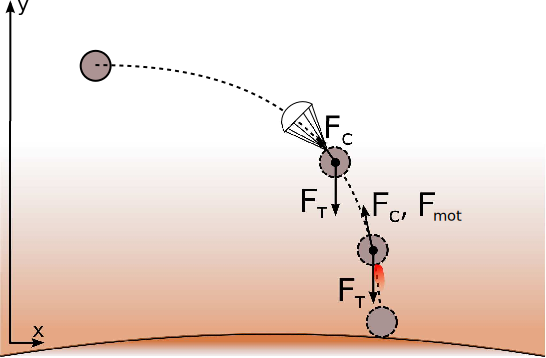
\includegraphics[width=8cm]{images/mars1-en.eps}
    \caption{Mars Landing Scheme}
    \label{Pic:mars}
  \end{center}
\end{figure}

Compared to the Moon, the task becomes more complicated: now you have to work in two dimensions (albeit in flat coordinates). The spacecraft has an initial horizontal (orbital) speed. In addition, now the spacecraft is affected not only by gravity, but also by the aerodynamic drag force (Stokes), proportional to the square of its speed. All this makes the analytical solution very difficult, so we suggest that you qualitatively evaluate the values of velocities and forces, as well as carefully analyze the results of unsuccessful flights.

\subsection{Initial data}

\begin{center}
\begin{tabular}{ |c|p{6.5cm}|p{6cm}| }
  \hline
  \textbf{Parameter} & \textbf{Explanation} & \textbf{Value} \\
  \hline
  $ G $ & Gravitational constant & $ 6.6742 \cdot 10^{-11} \text{H} \text{m}^{2}/\text{kg}^{2} $ \\
   \hline
   $ M $ & Mass of Mars & $6.4185 \cdot 10^{23} \text{kg}$ \\
   \hline
   $ R $ & Radius of Mars & \emph{3 389 500 m (3389.5 km)} \\
   \hline
   $ H $ & Launch orbit altitude & \emph{80,000 m} \\
   \hline
   $ k $ & Aerodynamic coefficient. Known for spherical spacecraft & 0.47 \\
   \hline
   $ S $ & Characteristic area of the body
   heat shield or parachute if deployed) & calculated as $ S = \pi r $, where $r$~--- radius
   machine \\
   \hline
   $ r $ & Spacecraft radius & \emph{0.811 m} \\
   \hline
   $ m $ & Mass of the spacecraft (at the beginning of the flight) & \emph{1397.61 kg} \\
   \hline
   $ v $ & Launch spacecraft speed (horizontal) & \emph{3555.07 m/s} \\
   \hline
   $ F_{\text{mot}} $ & Lander Force &
   Calculated using the formula: $ F_{\text{mot}} = u \cdot \Delta m$.\\
   \hline
   $ u $ & Velocity of outflow of gases from the engine nozzle & \emph{3600 m/s}\\
   \hline
   $ \Delta m $ & Thrust (fuel consumption) & \emph{4.2 kg/s}, craft equipped with \emph{50 kg}
   fuel\\
   \hline
   $ V_{\text{damping}}$ & Speed limit for damping & \emph{40 m/s} \\
   \hline
\end{tabular}
\end{center}

The machine is equipped with the following main devices:

\begin{center}
\begin{tabular}{ |p{5cm}|c|p{8.5cm}| }
   \hline
   \textbf{Name} & \textbf{Code} & \textbf{Destination} \\
   \hline
   Air Brake (Heat Shield) & \textbf{Hsl1} & Applied upon re-entry. This massive shield is used to dampen the spacecraft's main speed. \\
   \hline
   Rarefied Atmosphere Parachute & \textbf{Pam1} & Huge area parachute allows you to slow down the craft even in a rarefied atmosphere.\\
   \hline
   Landing Engine & \textbf{EG1} & An engine with low thrust that allows you to adjust the landing speed of the spacecraft. \\
   \hline
   Damper & \textbf{Dm1} & Damper allows you to absorb excess speed when reaching the surface. Here we consider a simplified version of work with a damper based on the limiting speed, a more accurate calculation can be made based on the absorption of kinetic energy by the damper, as described in the description of the next mission\\
   \hline
\end{tabular}
\end{center}

Each device can be \textbf{turned on} or \textbf{turned off} (using the <<TURNON>> and <<TURNOFF>> commands or the corresponding calls in a Python program), specifying the turn-on or turn-off time in seconds from the start of landing, respectively.

Please note that:

\begin{itemize}
   \item the parachute has a maximum speed limit~--- if the parachute is opened too early, it will simply be torn off (see table below);
   \item when the parachute or aerodynamic brake is turned off, they are discarded, which means that their mass (see the table below) is subtracted from the mass of the spacecraft, and it will not be possible to turn on these devices several times;
   \item \emph{cannot} open the parachute before the airbrake has been released~--- they will become entangled and both of them will be torn off;
   \item parachute or airbrake \emph{can} be used in conjunction with the engine;
   \item the landing engine consumes fuel, the spacecraft is equipped with a fuel tank for \emph{50 kg} of fuel;
   \item when landing the spacecraft, the engine is switched off automatically.
\end{itemize}

Another limitation that appears on Mars in connection with landing in the atmosphere is the maximum overload of the spacecraft. If the spacecraft's acceleration exceeds \emph{155 $\text{m}/\text{s}^2$}, it will be destroyed by overload.

Parachute and aerodynamic brake parameters:

\begin{center}
\begin{tabular}{ |p{5cm}|c|c|c|p{3cm}| }
   \hline
   \textbf{Name} & \textbf{Code} & \textbf{Area, $\text{m}^2$} & \textbf{Mass, kg} &
   \textbf{Maximum speed, m/s} \\
   \hline
   Aerobrake & \textbf{Hsl} & 18 & 150 & 7000 \\
   \hline
   Rarefied Air Parachute & \textbf{Pam} & 200 & 10 & 600 \\
   \hline
\end{tabular}
\end{center}

You can see the limitations of the physical model that is used when landing on Mars in the \ref{Sec:Mars-Model} appendix.

\subsection{Step one. Understanding Gravity Model Calculations}

To land on Mars, we will have to use a lot of the program for calculations on Earth. The calculation program allows you to get the trajectory of free fall of a body with given parameters on the surface of Mars (taking into account the used physical model of gravity, atmosphere, etc.).

The design of the spacecraft is fixed, so let's start with the known parameters:

\begin{itemize}
   \item characteristic body area: \emph{2.0663 $\text{m}^2$};
   \item mass: \emph{1397.61 kg};
   \item start position ($x$): \emph{0 m};
   \item starting altitude ($y$): \emph{80,000 m};
   \item starting horizontal speed ($V_x$): \emph{3555.0733 m/s};
   \item starting vertical speed ($V_y$): \emph{0 m/s}.
\end{itemize}

\hfill

\noindent\fbox{\parbox{\textwidth}{%
Enter the known initial values into the program and determine the speed of the spacecraft at the moment it touches the surface. Will this speed be compensated by the damper?
}}

\hfill

The output of the gravity model is approximately the following data set:

\begin{verbatim}
Ti=00 X=0000000.0 H=080000.0 Vx=3555.1 Vy=00000.0 Ang=00.0 Ac=003.6 As=000.2
Ti=10 X=0035896.5 H=079816.7 Vx=3553.2 Vy=-0035.9 Ang=00.6 Ac=003.6 As=000.2
Ti=20 X=0071063.2 H=079284.8 Vx=3551.2 Vy=-0071.2 Ang=01.1 Ac=003.6 As=000.2
...
\end{verbatim}

The output parameters will repeat the already familiar log of the flight of the device on the Moon. In addition to the coordinates and velocity components, the log contains the angle relative to the starting horizontal flight (\textbf{Ang}), the absolute values of the total spacecraft acceleration (\textbf{Ac}) and the spacecraft acceleration associated with the aerodynamic drag force (\textbf{Adf}). Examples of graphs of the gravity model are shown in the figure:

\begin{figure}[tbh]
  \begin{center}
    \includegraphics[width=16cm]{images/gravitymodel.eps}
    \caption{Presentation of gravity model results}
    \label{Pic:gravitymodel}
  \end{center}
\end{figure}

The free fall of the spacecraft leads to disaster. What to do?

Let's take a look at the available equipment~--- actually, from the start, the heat shield (\textbf{Hsl1}) is enabled. Our calculation did not take this into account, because the heat shield increases the effective area by \textbf{18 $\text{m}^2$}.

\hfill

\noindent\fbox{\parbox{\textwidth}{%
Calculate the new characteristic area of the body as the sum of the area of the spacecraft and the area of the heat shield. How has the calculated landing speed changed? Is just a heat shield and damper sufficient for a successful landing?
}}

\subsection{Step two. What to use - engine or parachute?}

To somehow slow down the descent, you need to look at the equipment of the spacecraft. From suitable equipment, we have engines and a parachute.

Engines are characterized by jet speed (in this case \emph{3600 m/s}) and power, which is proportional to fuel consumption (in our case \emph{4.2 kg/s}). Let's make a rough estimate of our ability to slow down the fall with engines.

We use the Tsiolkovsky formula for rocket speed:

$$
v = u \ln\left(\frac{M_1}{M_2}\right)
$$

where $u$~--- specific thrust (jet outflow velocity), $M_1$~--- mass of spacecraft with fuel, $M_2$~--- mass of spacecraft without fuel.

Substitute our values ($M_2$ will be obtained by subtracting the mass of fuel from the total mass) and get the speed that we will generate by the engine.

\hfill

\noindent\fbox{\parbox{\textwidth}{Will the speed calculated by the formula, obtained from the engines, be able to compensate for the acceleration of the spacecraft by gravity? (In reality, there will be even less benefit from the engine, as there is environmental resistance and other factors).
}}

\hfill

If the thrusters allow you to compensate for the fall speed (which we calculated in the previous step), you should use them when landing. Otherwise, use a parachute to further reduce speed.

\subsection{Step three. Parachute landing}

As you can see from the design of the spacecraft, it has a Low Atmosphere Parachute (\textbf{Pam1}). The following characteristics are important to us: area (\emph{200 $\text{m}^2$}) and maximum allowable speed (\emph{600 m/s}).

How to work with area~--- understandable. This is a value that is added to the characteristic area of the body and affects the aerodynamic drag force of our spacecraft.

The maximum allowable speed~--- is the speed that the parachute can withstand. If the speed of the air flow (it is the speed of our spacecraft) is greater, then the parachute will break.

So when do you open your parachute? On the one hand, the sooner~--- the better, the more time it will slow us down and the more the speed will decrease. On the other hand, if you open it at too high a speed, it will be blown away by the current.

Let's look at our calculation program. The spacecraft speed is the sum of the speeds $V_x$ and $V_y$. The resulting speed $V$ can be found using the Pythagorean theorem.

\hfill

\noindent\fbox{\parbox{\textwidth}{%
Use a calculation program to calculate at what minute will the parachute release speed be reached?
}}

\hfill

So we get a moment in time at which we can drop the heat shield and, at the same time, release the parachute.

\hfill

\noindent\fbox{\parbox{\textwidth}{%
Use the calculator again. But this time, calculate the last section of the trajectory~--- parachute descent. As initial conditions (speed, height) we need to take the result from the previous launch for the moment in time when we release the parachute. At what speed will the surface of the planet be touched now?
}}

\hfill

Do not forget that the parachute and the heat shield cannot be active at the same time, and also that the mass of the device will decrease by the mass of the discarded shield.
\hfill

\noindent\fbox{\parbox{\textwidth}{%
If the speed at the moment of touchdown is not enough to be compensated by the damper, can it be compensated by the motors? For this estimate, we have the limit speed obtained in the previous step.
}}

\subsection{Step four. Final brake}

Now we have to decide when to turn on (and off) the engines.

If we turn them on too soon, the spacecraft will stop at high altitude, and then when it runs out of fuel, it will fall and crash. If we turn it on late, the engines will not have time to slow down the spacecraft.

It is extremely difficult to solve this problem mathematically precisely, since the movement of our spacecraft, taking into account all the forces acting on it, is described by a complex differential equation. But some estimates can be made. To do this, we again use the Tsiolkovsky formula for jet propulsion.

Since we know what speed we need to extinguish (this is the speed at which we will collide with the surface if we do not turn on the engine), we can calculate the mass of fuel that we need to spend for this.

$$
\begin{array}{c}

  v = u \ln\left(\frac{M_1}{M_2}\right) \\
  \frac{v}{u} = \ln\left(\frac{M_1}{M_2}\right) \\
  e^{\frac{v}{u}} = \frac{M_1}{M_2}
\end{array}
$$

\hfill

\noindent\fbox{\parbox{\textwidth}{%
Using the Tsiolkovsky formula, estimate at what point you need to turn on the motor brake. Now you can design a spacecraft and go to Mars.
}}

\subsection{Physical model}
\label{Sec:Mars-Model}

The spacecraft is approaching Mars at a known height (80 km above the surface of the planet) with a known speed~--- the first space speed, which in turn is determined by the following formula:

$$
v = \sqrt{\frac{G \cdot M}{R}},
$$

where $G$~--- gravitational constant, $M$ and $R$~--- mass and radius of Mars.

For the sake of simplicity, we consider only a two-dimensional problem with the transition from a circle to a flat surface, so that the velocity is decomposed into two perpendicular components. At the beginning, the vertical velocity component ($Vy$) is equal to zero.

Further, the change in the parameters of the spacecraft is determined by the following differential equation:

$$
\frac{dv}{dt} = \frac{G M}{(R + y)^2} - \frac{k \rho(y) v^2 S}{2 m} - \frac{F_{\text{mot}}}{m}
$$

where $v$~-- is the spacecraft speed, $y$~-- is the height above the surface of Mars, $\rho(y)$~-- is the density of the Martian atmosphere depending on the height (exponential dependence), k~-- is the aerodynamic coefficient (the spacecraft has a spherical shape, it is known), $S$~-- is the cross-sectional area of the spacecraft, $m$~-- is the mass of the spacecraft, $F_{\text{dv}}$ is the force of the braking engines.

It can be seen that, in the general case, only three forces act on the spacecraft (gravitational, aerodynamic drag according to Stokes, and engines). In fact, this is how the formula for vertical movement looks like. When moving horizontally, the component of gravity will be equal to zero. This equation is given for scalar values, and the aerodynamic drag is always directed against the velocity vector, and the force of the engines~--- against the force of gravity.

The graph of the density of the atmosphere of Mars used in the model is shown in the figure.
\ref{Pic:mars_atmosphere}.

\begin{figure}[tbh]
  \begin{center}
    \includegraphics[width=10cm]{images/mars-atm.eps}
    \caption{Graph of changes in the density of the atmosphere of Mars}
    \label{Pic:mars_atmosphere}
  \end{center}
\end{figure}

The density of the Martian atmosphere varies from \textbf{0.026 $\text{kg}/\text{m}^3$} on the surface to approximately zero at \textbf{80,000 m}, where the spacecraft begins its descent.

\subsection{Telemetry analysis}

You have access to the spacecraft telemetry records for all completed flights. In addition to general information about the spacecraft, you will see a table of changes in the main parameters of the device over time:

\begin{verbatim*}
Ti=00:03:17 X=0616595.0 H=016504.3 Vx=2371.1 Vy=-0590.0
 Ac=13.74 Ae=000.0 As=016.2
...
\end{verbatim*}

Possible telemetry parameters are presented in the table:

\begin{center}
\begin{tabular}{ |c|c|p{2.5cm}|p{6cm}| }
  \hline
  \textbf{Name} & \textbf{Code} & \textbf{Unit} & \textbf{Comment} \\
   \hline
   Flight time & \textbf{Ti} & h:m:s & Telemetry period \emph{1 s}\\
   \hline
   Horizontal position & \textbf{X} & m & Initial position taken as \emph{0}\\
   \hline
   Height above ground & \textbf{H} & m & Initial height \emph{50,000 m}\\
   \hline
   Horizontal speed & \textbf{Vx} & m/s & Initial speed is equal to the first
   space for Mars\\
   \hline
   Vertical speed & \textbf{Vy} & m/s & Initial speed is
   \emph{0}. Recall that the $y$ axis is directed upward\\
   \hline
   Orientation angle of the spacecraft & \textbf{Ang} & ° & Angle of the spacecraft relative to the home position (0°-90°)\\
   \hline
   Total acceleration & \textbf{Ac} & $\text{m}/\text{c}^{2}$ & Absolute value of acceleration\\
   \hline
   Acceleration from engines & \textbf{Ae} & $\text{m}/\text{s}^{2}$ & Absolute value of acceleration,
   created by the included engine\\
   \hline
   Stokes Force Acceleration & \textbf{As} & $\text{m}/\text{s}^{2}$ & The absolute value of the acceleration,
   created by the force of aerodynamic resistance\\
  \hline
\end{tabular}
\end{center}

\section{Mercury}

Mercury is one of the mysterious planets in the solar system. With a seemingly small distance from the Earth, this planet is still rather poorly explored. The more interesting is the challenge~~--- to develop and land our own automatic station on Mercury.

Landing on Mercury is like landing on the Moon: no atmosphere, same vertical movement. However, this time you will have to fully develop the design of the spacecraft and its flight program on your own.

\begin{figure}[tbh]
  \begin{center}
    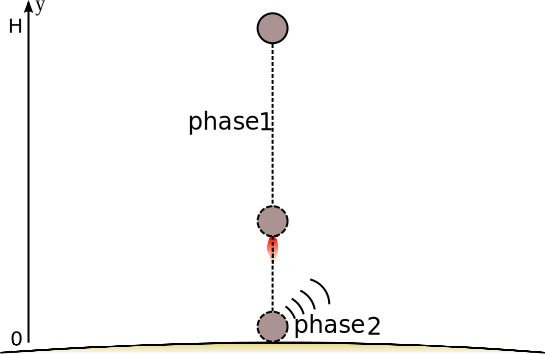
\includegraphics[width=8cm]{images/mercury-en.eps}
    \caption{Scheme of landing the spacecraft on Mercury}
    \label{Pic:mercury}
  \end{center}
\end{figure}

The spacecraft, which has reached the surface, will begin to transmit scientific results to Earth. The winner will be the one who will not only land the spacecraft on the surface of Mercury first, but will be able to equip the spacecraft with the maximum number of working scientific instruments.

\subsection{Initial data}

\begin{center}
\begin{tabular}{ |c|p{6.5cm}|p{6cm}| }
  \hline
  \textbf{Parameter} & \textbf{Explanation} & \textbf{Value} \\
   \hline
   $ G $ & Gravitational constant & $ 6.6742 \cdot 10^{-11} \text{H} \text{m}^{2}/\text{kg}^{2} $ \\
   \hline
   $ M $ & Mass of Mercury & $3.33 \cdot 10^{23} \text{kg}$ \\
   \hline
   $ R $ & Radius of Mercury & \emph{2 439 700 m (2439.7 km)} \\
   \hline
   $ \rho_c $ & Spacecraft density & \emph{100 $\text{kg}/\text{m}^3$} \\
   \hline
   $ F_{\text{mot}} $ & Lander Force &
   Calculated by the formula: $ F_{\text{mot}} = u \cdot \Delta m$, in which the ejection velocity
   and fuel consumption depend on the engine used.\\
  \hline
\end{tabular}
\end{center}

You do not have to design the spacecraft from scratch. You will have a spherical spacecraft at your disposal, the size of which you can set yourself. All you need to do is to choose the equipment and scientific instruments necessary for landing so that their total volume and the allowable mass of the device do not exceed the allowable values. You will also have to monitor the level of power supply in the spacecraft so that all systems have enough energy. In addition to the design of the device, you will also have to develop a flight program, for example, determine the time when the brake engines should turn on and off. When creating an spacecraft, it is necessary to take into account the maximum restrictions on the mass (\textbf{20 tons}) and the radius of the outer sphere (\textbf{2 m}).

\begin{figure}[tbh]
  \begin{center}
    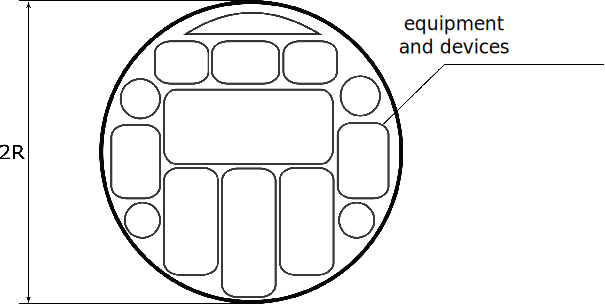
\includegraphics[width=10cm]{images/mercury-probe-en.eps}
    \caption{The design of the device on Mercury}
    \label{Pic:mercury-probe}
  \end{center}
\end{figure}

When landing on Mercury, the following engines and fuel tanks can be used:

\begin{center}
\begin{tabular}{ |p{2.5cm}|c|p{1.5cm}|p{1.5cm}|p{2cm}|p{2cm}|p{2.5cm}| }
  \hline
  \textbf{Name} & \textbf{Code} & \textbf{Mass, kg} & \textbf{Volume, $\text{m}^3$} &
   \textbf{Speed, m/s} & \textbf{Cons. energy, * 10 W} & \textbf{Parameter}\\
   \hline
   Brake engine & \textbf{E} & 1900 & 0.7 & 800 & 25 & Fuel consumption $\Delta m =
   0.5$~\emph{kg/s}\\
   \hline
   Landing engine & \textbf{EG} & 250 & 1.0 & 3600 & 5 & Fuel consumption $\Delta m =
   4.2$~\emph{kg/s}\\
   \hline
   Shunting engine & \textbf{EM} & 140 & 0.025 & 800 & 11 & Fuel consumption $\Delta m =
   0.02$~\emph{kg/s}\\
   \hline
   Fuel tank basic & \textbf{FT} & 50 & 0.04 & - & - & Amount of fuel: 50~kg\\
   \hline
   Fuel tank large & \textbf{FTL} & 500 & 0.4 & - & - & Fuel quantity: 500~kg\\
   \hline
\end{tabular}
\end{center}

You will also have two types of dampers available. Please note that in this mission you will need to calculate the kinetic energy absorbed by the dampers, which is discussed in more detail in the next section.

\begin{center}
\begin{tabular}{ |p{5.5cm}|c|p{1.5cm}|p{1.5cm}|p{4cm}| }
  \hline
  \textbf{Name} & \textbf{Code} & \textbf{Mass, kg} & \textbf{Volume, $\text{m}^3$} &
   \textbf{Absorbed energy, MJ}\\
   \hline
   Damper & \textbf{Dm} & 400 & 0.08 & 1.2\\
   \hline
   Damper with damper mounts & \textbf{DAM} & 1000 & 0.15 & 3\\
   \hline
\end{tabular}
\end{center}

Of course, for a real spacecraft, only engines and fuel tanks will not be enough. A list of other devices available for constructing the spacecraft is described below.

The mass of the device is the sum of the mass of the structure and the mass of all devices and can be calculated using the following formula:

$$
m = m_c + \sum\limits_{i}m_{d_i},
$$

where $m_c$~--- the mass of the structure, which is calculated by the formula $m_c = V \cdot \rho_c$, $V$~--- the volume of the spacecraft (calculated as the volume of the ball by the formula $V = \frac{4}{ 3}\pi
r^3$), $\rho_c$~--- known construction density; $m_{d_i}$~--- mass of a single spacecraft $i$.

\subsection{Physical model}

Unfortunately, here one cannot easily use the analytical solution obtained for the Moon. The mass of Mercury is large, which means that more fuel will be needed for the brake engines, so that the effect of fuel consumption on the equations of motion can no longer be neglected. Therefore, we have to consider the following differential equation:

$$
\frac{dv}{dt} = -g + \frac{F_{\text{дв}}}{m},
$$

where $v$~--- spacecraft speed, $g$~--- gravity acceleration for Mercury $\left(g = \frac{G M}{R^2}\right)$, $m$~—- - spacecraft mass, $F_{\text{motor}}$~--- brake motor force, which is calculated by the formula $F_{\text{mot}} = u \cdot \Delta m$, where $u$~- -- jet stream velocity, $\Delta m$~--- fuel consumption.

However, the analytical solution obtained on the Moon can also be applied here~--- with serious amendments to the fact that the actual solution will be even further from the analytical one.

Let us pay special attention to the refinement of the damper model. Each damper is characterized by the maximum kinetic energy that it can absorb during landing. Recall that the kinetic energy is calculated by the formula:

$$
E = \frac{m v^2}{2},
$$

where $m$~--- the mass of the spacecraft at the time of landing, $v$~--- the value of the velocity of the spacecraft at the moment of landing. If the spacecraft's kinetic energy does not exceed the damper rating, the landing will be successful.

\subsection{Providing the spacecraft with energy and a communication channel}

A spacecraft that could successfully land on the surface of Mercury will work for more than \textbf{30 minutes}~--- after that, the electronics will be disabled by solar radiation. During this time, the spacecraft should transmit to Earth as much scientific information as possible. To do this, several special scientific instruments (cameras, spectrometers, etc.) can be added to the design of the spacecraft, each device has certain parameters of energy consumption and the amount of information that it can consume / generate per unit of time. The battery can store energy if there is an excess of power in the network at the current moment, or give energy if the power of the generators is not enough.

Other devices (such as motors, transmitters, or a central computer) also consume energy. In the same way, the communication channel can be filled with other information, for example, telemetry of the spacecraft parameters. If at some point in time the total electricity consumption exceeds the power of the switched on generators, the spacecraft goes into a special protected mode (<<safe mode>>), in which its functionality is limited. When the spacecraft switches back to protected mode, it fails. When you add devices to the machine, you can choose which devices are specifically enabled or disabled in secure mode.

Each spacecraft is characterized by the following set of parameters:

\begin{itemize}
\item weight;
\item volume;
\item energy consumption (or energy production in the case of a generator);
\item volume of generated (for telemetry devices and scientific equipment) or transmitted (for transmitters) data;
\item critical temperature~--- the upper limit of the temperature at which the device fails.
\end{itemize}

Designers need to design the spacecraft in such a way that it can not only work for as long as possible, but also transmit the maximum amount of scientific information to Earth. For this, transmitters are used that have different bandwidth and other characteristics. The channel is filled with both scientific information from instruments and
telemetry data.

In fact, you have to solve an engineering problem by combining various devices and controlling their operation using a simple command system that includes:

\begin{itemize}
\item turn on the device (\verb'TURNON');
\item turn off the device (\verb'TURNOFF');
\item set the data transfer period (\verb'PERIOD'): the amount of data generated per second can be <<spread>> over the set period~--- this reduces the load on the channel, but slows down the data transfer to the Earth.
\end{itemize}

When the spacecraft lands, all engines are automatically switched off.

Each command runs at a specific time specified in the spacecraft's activity program.

The following table lists all the devices that provide spacecraft control, power, and communications. The central onboard computer must be present in any spacecraft~--- it provides control of the spacecraft, and energy and communication devices are described in the next section.

\begin{center}
\begin{tabular}{ |p{3cm}|c|p{1.5cm}|p{1.5cm}|p{2.5cm}|p{3cm}|p{1.5cm}| }
  \hline
  \textbf{Name} & \textbf{Code} & \textbf{Mass, kg} & \textbf{Volume, $\text{m}^3$} &
   \textbf{Cons. energy, * 10 W} & \textbf{Traffic consumption, Kbps / Transmission period,
     c} & \textbf{Crit. temp., K}\\
   \hline
   Central computer & \textbf{CPU} & 50 & 0.04 & 10 & - & 410 \\
   \hline
   Diagnostic basic & \textbf{D} & 25 & 0.01 & 2 & 1 / 1-3600 & 425 \\
   \hline
   Extended Diagnostics & \textbf{DA} & 80 & 0.02 & 10 & 2 / 1-3600 & 410\\
   \hline
   Radioisotope Generator & \textbf{G} & 200 & 0.04 & Produces 50 & - & 430\\
   \hline
   Battery & \textbf{Acm} & 70 & 0.02 & Capacity 400 $\text{W}\cdot\text{h}$& - & 360\\
   \hline
   Solar Cell & \textbf{Sbt} & 30 & 0.06 & Produces 10 & - & 380\\
   \hline
   Solar Extended & \textbf{Sbe} & 80 & 0.14 & Produces 32 & - & 380\\
   \hline
   Transmitter base & \textbf{T} & 30 & 0.01 & 4 & Generates 20 / 1 & 428\\
   \hline
   Broadband Transmitter & \textbf{WT} & 160 & 0.05 & 8 & Generates 100 / 1 & 380\\
   \hline
\end{tabular}
\end{center}

Solar panels convert the sun's energy into electrical energy. The power of the generated electricity can be calculated by the formula:

$$
P = P_d \cdot \left\{
  \begin{array}{c}
    1, \text{if}~0 \leqslant t < \frac{t_{\text{с}}}{2}\\
    0, \text{if}~\frac{t_{\text{с}}}{2} \leqslant t < t_{\text{с}},
  \end{array}
\right.
$$

where $P_d$~--- solar battery power (W), $t$~--- current time of day (hours), $t_{\text{s}}$~--- length of day on the planet in hours.

The figure \ref{Pic:solar} shows a typical generation schedule for solar panels in the model.

\begin{figure}[tbh]
  \begin{center}
    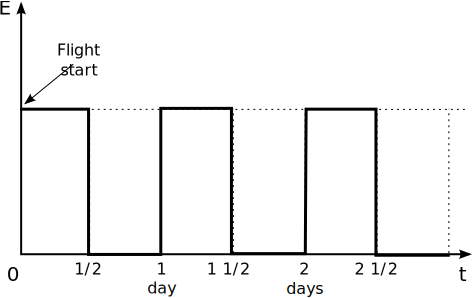
\includegraphics[width=8cm]{images/solar-graph-en.eps}
    \caption{Solar energy generation}
    \label{Pic:solar}
  \end{center}
\end{figure}

\subsection{Obtaining scientific data on the planet and determining the winner}

The result of the operation of any spacecraft is the transmission to Earth of data produced by scientific instruments. Several devices of the same type can be installed on the spacecraft~--- if there is enough power and bandwidth, they will all transmit the collected scientific information. At the same time, scientific information from devices of the same type is taken into account only until the corresponding limit is reached (information of this type becomes no longer interesting on Earth and is not taken into account when calculating victory points).

The following table lists all scientific instruments:

\begin{center}
\begin{longtable}{ |p{3cm}|c|p{1.5cm}|p{1.5cm}|p{1.5cm}|p{2cm}|p{1.5cm}|p{1.5cm}| }
  \hline
 \textbf{Name} & \textbf{Code} & \textbf{Mass, kg} & \textbf{Volume, $\text{m}^3$} &
   \textbf{Cons. energy, * 10 W} & \textbf{Cons. traffic, Kbps / Transmission period,
     c} & \textbf{Crit. temp., K} & \textbf{Scient. information, Gbit}\\
   \hline
   \endhead
   Camera & \textbf{C} & 10 & 0.005 & 14 & 18 / 1-100 & 345 & 0.7\\
   \hline
   Camcorder & \textbf{VC} & 20 & 0.008 & 34 & 27 / 1-10 & 330 & 0.8\\
   \hline
   Infrared Camera & \textbf{IRC} & 10 & 0.004 & 20 & 15 / 1-100 & 290 & 3\\
   \hline
   Radiometer & \textbf{Rm} & 14 & 0.02 & 8 & 10 / 1-100 & 400 & 1.2\\
   \hline
   Magnetic field sensor & \textbf{Mgm} & 10 & 0.003 & 9 & 9 / 1-10 & 380 & 1.5\\
   \hline
   Atmospheric laser analyzer & \textbf{LID} & 15 & 0.005 & 6 & 8 / 1-10 & 350 &
   2\\
   \hline
   Seismograph & \textbf{Smg} & 55 & 0.008 & 2 & 11 / 1-10 & 370 & 3.5\\
   \hline
   Barometer & \textbf{Brm} & 8 & 0.003 & 2 & 3 / 1-10 & 340 & 1\\
   \hline
   Thermometer & \textbf{Trm} & 2 & 0.003 & 2 & 2 / 1-10 & 450 & 0.5\\
   \hline
   Gas Chromatograph & \textbf{GCh} & 105 & 0.06 & 9 & 25 / 1-10 & 330 & 5.5\\
   \hline
   Speck\-ro\-fo\-to\-meter & \textbf{SPh} & 80 & 0.025 & 7 & 3 / 1-10 & 330 & 2.55\\
   \hline
   Laser Sample Evaporator & \textbf{LEv} & 20 & 0.025 & 80 & 98 / 1-10 & 380 & 1\\
   \hline
   Anemometer & \textbf{AN} & 12 & 0.003 & 4 & 1 / 1-10 & 390 & 1.35 \\
   \hline
   Spectrometer & \textbf{S} & 180 & 0.04 & 28 & 50 /1-100 & 350 & 4.6\\
   \hline
   Mass spectrometer & \textbf{MSS} & 200 & 0.08 & 19 & 22 / 1-100 & 310 & 7\\
   \hline
\end{longtable}
\end{center}

The winner is the constructor of the spacecraft that was able to transmit to Earth the maximum total amount of scientific information with the minimum starting mass of the spacecraft. That is, the number of victory points~--- the ratio of the received scientific information to the mass of the spacecraft.

\subsection{Telemetry analysis}

You have access to the telemetry records of the spacecraft from all completed flights. \textbf{Important:} The spacecraft's telemetry will be received on Earth if the spacecraft has a diagnostic device, a transmitter, and sufficient power. In addition to general information about the spacecraft, you will see a table of changes in the main parameters of the spacecraft over time.

Telemetry during the flight looks like this:

\begin{verbatim*}
Ti=00:00:01 H=099997.7 Vy=-0003.8 Ac=03.45 Ae=000.0
...
\end{verbatim*}

Possible telemetry parameters are presented in the table:

\begin{center}
\begin{tabular}{ |c|c|p{2.5cm}|p{6cm}| }
  \hline
  \textbf{Name} & \textbf{Code} & \textbf{Unit} & \textbf{Comment} \\
   \hline
   Flight time & \textbf{Ti} & h:m:s & Telemetry period \emph{1 s}\\
   \hline
   Height above ground & \textbf{H} & m & Initial height \emph{100,000 m}\\
   \hline
   Vertical speed & \textbf{Vy} & m/s & Initial speed is
   \emph{0}. Recall that the $y$ axis is directed upward\\
   \hline
   Total acceleration & \textbf{Ac} & $\text{m}/\text{c}^{2}$ & Absolute value of acceleration\\
   \hline
   Acceleration from engines & \textbf{Ae} & $\text{m}/\text{s}^{2}$ & Absolute value of acceleration,
   created by the included engine\\
   \hline
\end{tabular}
\end{center}

Telemetry after landing looks like this:

\begin{verbatim*}
Ti=00:01:30 PB=058 BW=10.1/20.0 SI=1000.0
...
\end{verbatim*}

The telemetry of the spacecraft after landing can also be analyzed in the form of graphs (see figure
\ref{Pic:telemetry-2}).

\begin{figure}[tbh]
  \begin{center}
    \includegraphics[width=16cm]{images/telemetry-2.eps}
    \caption{Presentation of spacecraft telemetry results}
    \label{Pic:telemetry-2}
  \end{center}
\end{figure}

Possible telemetry parameters are presented in the table:

\begin{center}
\begin{tabular}{ |c|c|p{2.5cm}|p{6cm}| }
  \hline
  \textbf{Name} & \textbf{Code} & \textbf{Unit} & \textbf{Comment} \\
   \hline
   Time of flight & \textbf{Ti} & h:m:s & Telemetry period \emph{1 s} (may be
   changed by command \verb'PERIOD')\\
   \hline
   Energy balance & \textbf{PB} & 10 W & Total energy production minus total energy
   spacecraft consumption\\
   \hline
   Communication channel & \textbf{BW} & Kbps & Used / Available communication channel\\
   \hline
   Scientific Information & \textbf{SI} & Kbps & Volume of Scientific Information Transferred\\
   \hline
\end{tabular}
\end{center}

When you turn on the <<Advanced Diagnostics>> device, you can get other spacecraft settings and information about the status of all devices.

\section{Venus}

Exploration of Venus~--- a real challenge for mankind. This planet is close in size to the Earth, has a dense atmosphere and a huge temperature on the surface. Here it is important not only not to crash on the surface, but also not to burn out when entering the dense layers of the atmosphere, and also to work on the surface at a temperature of 450 ° Celsius for as long as possible, transmitting data from scientific instruments to Earth.

In this task, everything will be real: you will have to design your own spacecraft and write a flight program for it. This time, it is necessary to take into account not only the volume and weight of the devices, but also how much insulator and heat sink must be placed in the spacecraft.

\begin{figure}[tbh]
  \begin{center}
    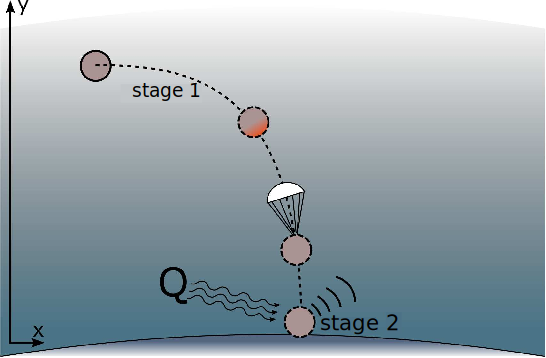
\includegraphics[width=8cm]{images/venus-en.eps}
    \caption{Venus Landing Scheme}
    \label{Pic:venus}
  \end{center}
\end{figure}

The winner here will be the one who can land the spacecraft on the surface of the planet and transmit to Earth as much scientific information as possible.

\subsection{Design of the device}

The general design of the spacecraft shown in the figure \ref{Pic:venus-probe} is close to that which we used on Mercury, but there are important differences. Firstly, all the free space between the devices is filled with a special heat sink. Secondly, you can set the outer and inner radius, the volume between which is filled with an insulator. So you can vary the size of the spacecraft~--- and hence the possible amount of payload,~--- and the resistance of the internal part of the spacecraft to external heat.

\begin{figure}[tbh]
  \begin{center}
    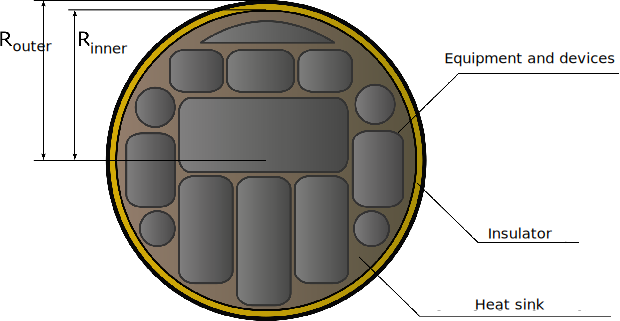
\includegraphics[width=10cm]{images/venus-probe-en.eps}
    \caption{The design of the spacecraft on Venus}
    \label{Pic:venus-probe}
  \end{center}
\end{figure}

\subsection{Physical model at the first stage: landing on the planet}

The mathematical model used in this problem is close to that used when landing on Mars, only under the conditions of Venus the influence of the planet's atmosphere will be much more significant.

The spacecraft is approaching Venus at a known altitude (\textbf{250 km} above the planet's surface) with a known speed~--- \textbf{half} of the first cosmic velocity, which in turn is determined by the following formula.

$$
v = \sqrt{\frac{G \cdot M}{R}},
$$

where $G$~--- gravitational constant, $M$ and $R$~--- mass and radius of Venus.

For the sake of simplicity, we consider only a two-dimensional problem with the transition from a circle to a flat surface, so that the velocity is decomposed into two perpendicular components, and at the beginning the vertical component of the velocity ($V_y$) is equal to zero.

Further, the change in the parameters of the spacecraft is determined by the following differential equation:

$$
\frac{dv}{dt} = \frac{G M}{(R + y)^2} - \frac{k \rho(y) v^2 S}{2 m} - \frac{F_{\text{mot}}}{m}
$$

where $v$~-- is the speed of the spacecraft, $y$~-- is the height above the surface of Mars, $\rho(y)$~-- is the density of the atmosphere of Venus depending on the height (exponential dependence), k~-- —
aerodynamic coefficient (the spacecraft has a spherical shape, it is known), $S$~-- is the cross-sectional area of the spacecraft, $m$~-- is the mass of the spacecraft, $F_{\text{mot}}$ is the force of the braking engines.

It can be seen that, in the general case, only three forces act on the spacecraft (gravitational, aerodynamic drag according to Stokes, and engines). In fact, this is how the formula for vertical movement looks like. When moving horizontally, the component of gravity will be equal to zero. This equation is given for scalar quantities, and the aerodynamic drag is always directed against the velocity vector, and the force of the engines~-- against the force of gravity.

The mass of the spacecraft consists of the mass of the structure, the mass of the insulator and absorber, the mass of all devices installed on the spacecraft. Mass can be calculated using the following formula:

$$
m = m_{\text{s}} + m_{\text{ins}} + m_{\text{abs}} + \sum\limits_{i}m_{\text{у}_i}
$$,

Where:

\begin{itemize}
   \item $m_{\text{s}}$~--- mass of the structure, which is calculated by the formula $m_{\text{s}} = V_{\text{inner}} \cdot \rho_{\text{s}}$, where $V_{\text{inner}}$~--- the volume of the inner sphere of the spacecraft (calculated as the volume of the ball using the formula $V = \frac{4}{3} \pi r^3$), $ \rho_{\text{s}}$~--- known construction density;
   \item $m_{\text{ins}}$~--- mass of the insulator, which is calculated by the formula $m_{\text{ins}} = (V_{\text{outer}} - V_{\text{inner} }) \cdot \rho_{\text{ins}}$, where $V_{\text{outer}}$ and $V_{\text{inner}}$~--- volumes of the external and internal spheres of the device, respectively, $ \rho_{\text{ins}}$~--- known insulator density;
   \item mass of the absorber, which is calculated by the formula $m_{\text{abs}} =
      \left(V_{\text{inner}} - \sum\limits_{i}V_{\text{у}_i}\right)\cdot \rho_{\text{abs}}$, where $V_{\text{у}_i}$~--- volume of a single device $i$,
       $\rho_{\text{abs}}$~--- known absorber density;
   \item $m_{\text{y}_i}$~--- the mass of a single device $i$.
\end{itemize}

When creating an spacecraft, it is necessary to take into account the maximum restrictions on the mass and radius of the outer sphere of the spacecraft: \textbf{20 tons} and \textbf{2 m}, respectively.

All parameters necessary for calculations are presented in the table:

\begin{center}
\begin{tabular}{ |c|p{6.5cm}|p{6cm}| }
  \hline
  \textbf{Parameter} & \textbf{Explanation} & \textbf{Value} \\
   \hline
   $ G $ & Gravitational constant & $ 6.6742 \cdot 10^{-11} \text{H} \text{m}^{2}/\text{kg}^{2} $ \\
   \hline
   $ M $ & Mass of Venus & $4.8685 \cdot 10^{24} \text{kg}$ \\
   \hline
   $ R $ & Radius of Venus & \emph{6 051 800 m (6052 km)} \\
   \hline
   $ k $ & Aerodynamic coefficient. Known for spherical spacecraft & 0.47 \\
   \hline
   $ S $ & Sectional area of the spacecraft, (increased by the area
   heat shield or parachute if deployed) & is calculated as $ S = \pi r $,
   where $r$~--- outer radius
   spacecraft \\
   \hline
   $ V $ & The volume of the inner and outer spheres of the spacecraft & Calculated as the volume of the ball using the formula $V = \frac{4}{3} \pi
     r^3$, where $r$~--- the corresponding radius of the spacecraft\\
   \hline
   $ \rho_{\text{s}} $ & spacecraft design density & \emph{400 $\text{kg}/\text{m}^3$} \\
   \hline
   $ \rho_{\text{ins}} $ & Insulator Density & \emph{4000 $\text{kg}/\text{m}^3$} \\
   \hline
   $ \rho_{\text{abs}} $ & Heat absorber density & \emph{1570 $\text{kg}/\text{m}^3$} \\
   \hline
   $ F_{\text{mot}} $ & Lander Force &
   Calculated using the formula: $ F_{\text{mot}} = u \cdot \Delta m$.\\
   \hline
\end{tabular}
\end{center}

For each of the devices used, the on and off times can be specified. Please note that:

\begin{itemize}
   \item the parachute has a maximum speed limit - if the parachute is opened too early, it will simply be torn off;
   \item when the parachute or aerodynamic brake is turned off, it is discarded, which means that its mass is subtracted from the mass of the spacecraft; also it will not be possible to turn on such a device several times;
   \item you can't open multiple parachutes at the same time~--- they will get tangled up and blown off;
   \item engines consume fuel; the spacecraft can be equipped with fuel tanks, the fuel from which is produced evenly;
   \item when the spacecraft lands, all engines and parachutes are automatically switched off.
\end{itemize}

Another limitation that Venus has in connection with landing in the atmosphere is ~ --- the maximum overload of the spacecraft. If the spacecraft's acceleration exceeds \textbf{115 $\text{m}/\text{s}^2$},
it will be destroyed by overload.

Devices used in landing on Venus can be divided into three groups: engines, heat shields / parachutes and dampers. When landing on Venus, the following engines and fuel tanks can be used:

\begin{center}
\begin{tabular}{ |p{2.5cm}|c|p{1.5cm}|p{1.5cm}|p{2cm}|p{2cm}|p{2.5cm}| }
  \hline
 \textbf{Name} & \textbf{Code} & \textbf{Mass, kg} & \textbf{Volume, $\text{m}^3$} &
   \textbf{Speed, m/s} & \textbf{Cons. energy, * 10 W} & \textbf{Parameter}\\
   \hline
   Brake engine & \textbf{E} & 1900 & 0.7 & 800 & 25 & Fuel consumption $\Delta m =
   0.5$~\emph{kg/s}\\
   \hline
   Landing engine & \textbf{EG} & 250 & 1.0 & 3600 & 5 & Fuel consumption $\Delta m =
   4.2$~\emph{kg/s}\\
   \hline
   Light landing engine & \textbf{EL} & 100 & 0.5 & 3600 & 5 & Fuel consumption $\Delta m =
   2$~\emph{kg/s}\\
   \hline
   Shunting engine & \textbf{EM} & 140 & 0.025 & 800 & 11 & Fuel consumption $\Delta m =
   0.02$~\emph{kg/s}\\
   \hline
   Fuel tank basic & \textbf{FT} & 50 & 0.04 & - & - & Amount of fuel: 50~kg\\
   \hline
   Fuel tank large & \textbf{FTL} & 500 & 0.4 & - & - & Fuel quantity: 500~kg\\
   \hline
\end{tabular}
\end{center}

Parameters of permissible parachutes and aerodynamic brake:

\begin{center}
\begin{tabular}{ |p{4cm}|c|p{2cm}|c|c|p{2cm}|p{2cm}| }
   \hline
   \textbf{Name} & \textbf{Code} & \textbf{Area, $\text{m}^2$} & \textbf{Mass, kg} &
   \textbf{Volume, $\text{m}^3$} &\textbf{Top speed, m/s} \\
   \hline
   Aerodynamic brake reinforced & \textbf{Hs} & 3 & 1000 & 0.01 & 4000 \\
   \hline
   Power parachute & \textbf{Fp} & 2 & 70 & 0.02 & 500\\
   \hline
   Parachute & \textbf{Pa} & 10 & 40 & 0.02 & 35 \\
   \hline
\end{tabular}
\end{center}

Please note that the included heat shield also allows you to reduce the heating of the spacecraft during landing, which will be discussed in the \ref{Sec:thermal} section.

Also, you will have access to only one type of damper:

\begin{center}
\begin{tabular}{ |p{5.5cm}|c|p{1.5cm}|p{1.5cm}|p{4cm}| }
  \hline
  \textbf{Name} & \textbf{Code} & \textbf{Mass, kg} & \textbf{Volume, $\text{m}^3$} & \textbf{Absorbed energy, MJ}\\
   \hline
   Damper & \textbf{Dm} & 400 & 0.08 & 1.2\\
  \hline
\end{tabular}
\end{center}

The density of the Venusian atmosphere is shown in \ref{Pic:venus atmosphere}.

\begin{figure}[tbh]
  \begin{center}
    \includegraphics[width=15cm]{images/venus-atm.eps}
    \caption{Graphs of changes in the density of the atmosphere of Venus depending on the height}
    \label{Pic:venus_atmosphere}
  \end{center}
\end{figure}

The density of the Venusian atmosphere varies from \textbf{67 $\text{kg}/\text{m}^3$} at the surface to approximately zero at about 100,000 m, where the dense layers of the atmosphere begin. Above \textbf{150 km}, the density of the Venusian atmosphere can already be neglected.

\subsection{Physical model at the second stage: work on the surface of the planet} \label{Sec:thermal}

In addition to direct landing on Venus, external temperature effects must be taken into account. When braking against the atmosphere, the spacecraft experiences thermodynamic heating. To simplify, we begin to consider this process from the moment when the density of the atmosphere exceeds \textbf{0.3 $\text{kg}/\text{m}^3$}. The temperature of the external circuit of the spacecraft is calculated by the formula:

$$
T_{\text{outer}} = T(y) + \frac{k v^2}{2 C},
$$

where $T(y)$~-- is the temperature of the atmosphere at height $y$ (in our model it increases linearly), $v$~-- is the spacecraft velocity, $C$~-- is the specific heat of the atmosphere of Venus (for simplification is treated as a constant), and $k$~-- is a special atmospheric coefficient, which is equal to $k = \frac{\rho(y)^{0.5}}{10}$, where $\rho(y) $~-- is the density of the atmosphere of Venus as a function of altitude.

A graph of the dependence of the temperature of the atmosphere of Venus on height is shown in the figure \ref{Pic:venus_temp}.

\begin{figure}[tbh]
  \begin{center}
    \includegraphics[width=10cm]{images/venus-temp.eps}
    \caption{Graph of temperature changes in the atmosphere of Venus}
    \label{Pic:venus_temp}
  \end{center}
\end{figure}

The temperature on the planet's surface is taken as \textbf{734 K}.

The transfer of heat from an external source (Venusian atmosphere) to the spacecraft is described by the following equation from thermodynamics. The initial temperature of the spacecraft is known, and then it heats up as it descends through the atmosphere and while on the hot surface.

For the time quantum $dt$, the following amount of heat is transferred to the spacecraft:

$$
dQ = -k \frac{\Delta T}{\Delta x} D dt,
$$

where $k$~-- is the heat absorption coefficient calculated by the formula $k = k_{\text{ins}} (1 - k_{\text{shield}})$, where $k_{\text{ins}}$ ~--- coefficient of thermal conductivity of the insulator, and $k_{\text{shield}}$~--- coefficient of heat absorption of the thermal shield (if the spacecraft has one), $S$~--- heat transfer surface area (sphere area), $ \frac{\Delta T}{\Delta x}$~--— the temperature gradient, which we consider linearly: we know the temperature difference~--— of the inner (absorber temperature) and outer (Venus atmosphere temperature), as well as the distance between the inner and outer sphere of the spacecraft (where the insulator is located).

Further, the heat is transferred to the so-called heat accumulator (heat sink), based on lithium nitrate hydrate. For this substance, the melting point is known, as well as the values of the heat capacity in the solid and liquid state. The next task is divided into three phases:

\begin{description}

\item[Solid heat sink heating] Heating occurs according to the following formula:

\begin{eqnarray}
T(t) = T_0 + \frac{Q}{C_{\text{solid}}m} = T_0 + \frac{Q}{C_{\text{solid}}\rho V}, \label{Eq:temp}
\end{eqnarray}

where $T_0$~--- the initial temperature of the device\footnote{For simplicity, the device does not track the lower temperature limit required for the operation of devices,~--- it is assumed that devices can operate even at a sufficiently low temperature.}, $C_ {\text{solid}}$~-- is the heat capacity of the heat sink in the solid state (constant), $\rho$~-- is the density of the absorber (constant), $V$~-- is the volume of the absorber, which is calculated as the difference between the volume of the internal sphere of the spacecraft and the total volume of all devices.

\item[Heat absorber melting] Until the entire absorber is melted, we consider the temperature throughout the entire internal volume of the spacecraft to be constant. The mass of the expanded absorber per unit time dt is calculated as:

  $$
dm = \frac{Q(t)dt}{L},
$$

where $L$~--- specific heat of melting of the heat sink.

\item[Liquid heat sink heating] The temperature change occurs similarly to the \ref{Eq:temp} formula, only $C_{\text{liquid}}$~--- heat capacity of the heat sink in the liquid state appears in the equation (we consider it a constant).

\end{description}

All three phases of spacecraft heating are clearly visible on the telemetry graph of the spacecraft on Venus (see figure \ref{Pic:venus_telemetry_temp}).

\begin{figure}[tbh]
  \begin{center}
    \includegraphics[width=10cm]{images/telemetry-temp.eps}
    \caption{Graph of temperature changes during landing on Venus and on its surface}
    \label{Pic:venus_telemetry_temp}
  \end{center}
\end{figure}

Each device inside the spacecraft has its own critical temperature. As soon as the temperature of the spacecraft rises to this level, the device burns out and no longer functions. The spacecraft actually ceases to function as soon as the Central computer fails.

Thus, players need to construct such a spacecraft that can continue its work on the surface of Venus as long as possible. In order to find the optimal solution to this problem, the participants will have to calculate the time that will be spent on each of the described phases. If for the second phase the time is calculated from a simple linear
equations, then for the first and third phases the differential equation does not have the simplest analytical solution, since it is inhomogeneous:

$$
T(t) = T_0 + (T_{\text{Ven}} - T_0)\left(1 - e^{\frac{-k S t}{\Delta x C \rho_{\text{abs}} V}}\right),
$$

where $T_{\text{Ven}}$ is the temperature of the atmosphere of Venus, the values of other parameters are given in the table below. Knowing the critical temperature, we can obtain a formula for calculating the heating time of the spacecraft to the temperature $T$:

$$
t(T) = - \frac{\Delta x C \rho_{\text{abs}} V}{k S} \ln{\left(\frac{T_{\text{Ven}} -
    T}{T_{\text{Ven}} - T_0}\right)}.
$$

Thus, designers can vary the parameters of the spacecraft in order to achieve the maximum duration of its operation under the conditions of Venus. The larger the spacecraft, the more heat it receives (the higher the contact area), the heavier it is, but the more space it has for devices. On the other hand, the thicker the insulator layer, the less space for devices inside the spacecraft (the insulator is light, we neglect its mass), but the slower it heats up.

The values of all parameters required to solve the thermodynamic problem are presented in the table:

\begin{center}
\begin{tabular}{ |p{2cm}|p{8cm}|p{3cm}| }
  \hline
  \textbf{Parameter} & \textbf{Explanation} & \textbf{Value} \\
   \hline
   $ T_0 $ & Initial spacecraft temperature (before reentry) & \emph{10 K} \\
   \hline
   $ T_{\text{Ven}} $ & Surface temperature of Venus & \emph{734 K} \\
   \hline
   $ C $ & Specific heat of the atmosphere of Venus & \emph{0.8 $\frac{\text{m}^2}{\text{K}
       \text{c}^2}$} \\
   \hline
   $ k_{\text{ins}} $ & Insulator Thermal Conductivity & 0.04\\
   \hline
   $ k_{\text{shield}} $ & Thermal shield heat absorption coefficient (\textbf{Hs}) & 0.3333\\
   \hline
   $ T_{\text{melt}} $ & Heat sink melting point & \emph{303 K}\\
   \hline
   $ C_{\text{solid}}$ & Heat sink heat capacity in solid state & \emph{2435
     $\frac{\text{J}}{\text{kg} \cdot \text{K}}$}\\
   \hline
   $ C_{\text{liquid}}$ & Heat sink heat capacity in liquid state & \emph{4200
     $\frac{\text{J}}{\text{kg} \cdot \text{K}}$}\\
   \hline
   $ L $ & Specific heat of fusion of the heat sink & \emph{439 $\frac{\text{kJ}}{\text{kg}}$} \\
   \hline
\end{tabular}
\end{center}

\subsection{Providing the spacecraft with energy and a communication channel}

The main task of the spacecraft is to transmit scientific information to Earth. To do this, several special scientific devices (cameras, spectrometers, etc.) can be added to the design of the spacecraft, each of which has a certain power consumption and the amount of information that they are able to generate per unit time.

Other devices (such as running motors, transmitters, or a central computer) also consume power. In the same way, the communication channel can be filled with other information, for example, telemetry of the spacecraft parameters. If at some point in time the total electricity consumption exceeds the power of the switched on generators, the spacecraft goes into a special protected mode (<<safe mode>>), in which its functionality is limited. When the spacecraft switches back to protected mode, it fails. When you add devices to the machine, you can choose which devices are specifically enabled or disabled in secure mode.

Each device is characterized by the following set of parameters:

\begin{itemize}
\item weight;
\item volume;
\item energy consumption (or energy production in the case of a generator);
\item volume of generated (for telemetry devices and scientific equipment) or transmitted (for transmitters) data;
\item critical temperature~--- the upper limit of the temperature at which the device fails.
\end{itemize}

Designers need to design the spacecraft in such a way that it can not only work for as long as possible, but also transmit the maximum amount of scientific information to Earth. For this, transmitters are used that have different bandwidth and other characteristics. The channel is filled with both scientific information from instruments and telemetry data.

In fact, you have to solve an engineering problem by combining various devices and controlling their operation using a simple command system that includes:

\begin{itemize}
\item turn on the device (\verb'TURNON');
\item turn off the device (\verb'TURNOFF');
\item set the data transfer period (\verb'PERIOD'): the amount of data generated per second can be <<spread>> over the set period~--- this reduces the load on the channel, but slows down the data transfer to the Earth.
\end{itemize}

Each command runs at a specific time specified in the spacecraft's activity program.

The following table lists all the devices that provide spacecraft control, power, and communications. The central computer must be present in any spacecraft~--- it provides control of the spacecraft, and energy and communication devices are described in the next section.

\begin{center}
\begin{tabular}{ |p{3cm}|c|p{1.5cm}|p{1.5cm}|p{2.5cm}|p{3cm}|p{1.5cm}| }
  \hline
  \textbf{Name} & \textbf{Code} & \textbf{Mass, kg} & \textbf{Volume, $\text{m}^3$} &
   \textbf{Cons. energy, * 10 W} & \textbf{Traffic consumption, Kbps / Transmission period,
     c} & \textbf{Crit. temp., K}\\
   \hline
   Central computer & \textbf{CPU} & 50 & 0.04 & 10 & - & 410 \\
   \hline
   Diagnostic basic & \textbf{D} & 25 & 0.01 & 2 & 1 / 1-3600 & 425 \\
   \hline
   Extended Diagnostics & \textbf{DA} & 80 & 0.02 & 10 & 2 / 1-3600 & 410\\
   \hline
   Radioisotope Generator & \textbf{G} & 200 & 0.04 & Produces 50 & - & 430\\
   \hline
   Battery & \textbf{Acm} & 70 & 0.02 & Capacity 400 $\text{W}\cdot\text{h}$& - & 360\\
   \hline
   Transmitter base & \textbf{T} & 30 & 0.01 & 4 & Generates 20 / 1 & 428\\
   \hline
   Broadband Transmitter & \textbf{WT} & 160 & 0.05 & 8 & Generates 100 / 1 & 380\\
   \hline
\end{tabular}
\end{center}

On a mission to Venus, solar panels are not efficient, so they are not used.

\subsection{Obtaining scientific data on the planet and determining the winner}

The result of the operation of any spacecraft is the transmission to Earth of data produced by scientific instruments. Several devices of the same type can be installed on the spacecraft~--- if there is enough power and bandwidth, they will all transmit the collected scientific information. At the same time, scientific information from devices of the same type is taken into account only until the corresponding limit is reached (information of this type becomes no longer interesting on Earth and is not taken into account when calculating victory points).

The following table lists all scientific instruments:

\begin{center}
\begin{longtable}{ |p{3cm}|c|p{1.5cm}|p{1.5cm}|p{1.5cm}|p{2cm}|p{1.5cm}|p{1.5cm}| }
  \hline
 \textbf{Name} & \textbf{Code} & \textbf{Mass, kg} & \textbf{Volume, $\text{m}^3$} &
   \textbf{Cons. energy, * 10 W} & \textbf{Cons. traffic, Kbps / Transmission period,
     c} & \textbf{Crit. temp., K} & \textbf{Scient. information, Gbit}\\
   \hline
   \endhead
   Camera & \textbf{C} & 10 & 0.005 & 14 & 18 / 1-100 & 345 & 0.7\\
   \hline
   Camcorder & \textbf{VC} & 20 & 0.008 & 34 & 27 / 1-10 & 330 & 0.8\\
   \hline
   Infrared Camera & \textbf{IRC} & 10 & 0.004 & 20 & 15 / 1-100 & 290 & 3\\
   \hline
   Radiometer & \textbf{Rm} & 14 & 0.02 & 8 & 10 / 1-100 & 400 & 1.2\\
   \hline
   Magnetic field sensor & \textbf{Mgm} & 10 & 0.003 & 9 & 9 / 1-10 & 380 & 1.5\\
   \hline
   Atmospheric laser analyzer & \textbf{LID} & 15 & 0.005 & 6 & 8 / 1-10 & 350 &
   2\\
   \hline
   Seismograph & \textbf{Smg} & 55 & 0.008 & 2 & 11 / 1-10 & 370 & 3.5\\
   \hline
   Barometer & \textbf{Brm} & 8 & 0.003 & 2 & 3 / 1-10 & 340 & 1\\
   \hline
   Thermometer & \textbf{Trm} & 2 & 0.003 & 2 & 2 / 1-10 & 450 & 0.5\\
   \hline
   Gas Chromatograph & \textbf{GCh} & 105 & 0.06 & 9 & 25 / 1-10 & 330 & 5.5\\
   \hline
   Speck\-ro\-fo\-to\-meter & \textbf{SPh} & 80 & 0.025 & 7 & 3 / 1-10 & 330 & 2.55\\
   \hline
   Laser Sample Evaporator & \textbf{LEv} & 20 & 0.025 & 80 & 98 / 1-10 & 380 & 1\\
   \hline
   Anemometer & \textbf{AN} & 12 & 0.003 & 4 & 1 / 1-10 & 390 & 1.35 \\
   \hline
   Spectrometer & \textbf{S} & 180 & 0.04 & 28 & 50 /1-100 & 350 & 4.6\\
   \hline
   Mass spectrometer & \textbf{MSS} & 200 & 0.08 & 19 & 22 / 1-100 & 310 & 7\\
   \hline
\end{longtable}
\end{center}

The winner is the constructor of the spacecraft that was able to transmit to Earth the maximum total amount of scientific information with the minimum starting mass of the spacecraft. That is, the number of victory points~--- the ratio of the received scientific information to the mass of the spacecraft.

\subsection{Telemetry analysis}

You have access to the telemetry records of the spacecraft from all completed flights. \textbf{Important:} the spacecraft's telemetry will be received on Earth if the spacecraft has a diagnostic device,
transmitter and sufficient power. In addition to general information about the device, you will see a table of changes in the main parameters of the spacecraft over time.

Telemetry during the flight looks like this:

\begin{verbatim*}
Ti=00:00:10 X=0037003.8 H=249578.5 Vx=3663.7 Vy=-0082.6 Ang=01.3
   Ac=008.2 Ae=000.0 As=000.0 Te=010.0
Ti=00:00:20 X=0073274.8 H=248355.3 Vx=3663.7 Vy=-0163.7 Ang=02.5
   Ac=008.2 Ae=000.0 As=000.0 Te=010.0
Ti=00:00:30 X=0109912.3 H=246305.1 Vx=3663.7 Vy=-0245.6 Ang=03.8
   Ac=008.2 Ae=000.0 As=000.0 Te=010.0
...
\end{verbatim*}

Possible telemetry parameters are presented in the table:

\begin{center}
\begin{tabular}{ |p{5cm}|c|p{2.5cm}|p{6cm}| }
   \hline
   \textbf{Name} & \textbf{Code} & \textbf{Unit} & \textbf{Comment} \\
   \hline
   Flight time & \textbf{Ti} & h:m:s & Telemetry period \emph{1 s}\\
   \hline
   Horizontal position & \textbf{X} & m & Initial position taken as \emph{0}\\
   \hline
   Height above ground & \textbf{H} & m & Initial height \emph{50,000 m}\\
   \hline
   Horizontal speed & \textbf{Vx} & m/s & Initial speed is equal to the first
   space for Mars\\
   \hline
   Vertical speed & \textbf{Vy} & m/s & Initial speed is
   \emph{0}. Recall that the $y$ axis is directed upward\\
   \hline
   Orientation angle of the machine & \textbf{Ang} & ° & Angle of the spacecraft relative to the home position (0°-90°)\\
   \hline
   Total acceleration & \textbf{Ac} & $\text{m}/\text{c}^{2}$ & Absolute value of acceleration\\
   \hline
   Acceleration from engines & \textbf{Ae} & $\text{m}/\text{s}^{2}$ & Absolute value of acceleration,
   created by the included engine\\
   \hline
   Stokes Force Acceleration & \textbf{As} & $\text{m}/\text{s}^{2}$ & The absolute value of the acceleration,
   created by the force of aerodynamic resistance\\
   \hline
   spacecraft internal temperature & \textbf{Te} & K & Pre-entry temperature \emph{10K}\\
   \hline
\end{tabular}
\end{center}

Telemetry after landing looks like this:

\begin{verbatim*}
Ti=00:00:10 PB=070 BW=18.2/20.0 Te=303.0
Ti=00:00:20 PB=070 BW=18.2/20.0 Te=303.0
Ti=00:00:30 PB=070 BW=18.2/20.0 Te=303.0
Ti=00:00:40 PB=070 BW=18.2/20.0 Te=303.0
...
\end{verbatim*}

Possible telemetry parameters are presented in the table:

\begin{center}
\begin{tabular}{ |p{4cm}|c|p{2.5cm}|p{6cm}| }
  \hline
  \textbf{Name} & \textbf{Code} & \textbf{Unit} & \textbf{Comment} \\
   \hline
   Time of flight & \textbf{Ti} & h:m:s & Telemetry period \emph{1 s} (may be
   changed by command \verb'PERIOD')\\
   \hline
   Energy balance & \textbf{PB} & 10 W & Total energy production minus total energy
   spacecraft consumption\\
   \hline
   Communication channel & \textbf{BW} & Kbps & Used / Available communication channel\\
   \hline
   spacecraft internal temperature & \textbf{Te} & K & Pre-entry temperature \emph{10K}\\
   \hline
   Scientific Information & \textbf{SI} & Kbps & Volume of Scientific Information Transferred\\
   \hline
\end{tabular}
\end{center}

When you turn on the <<Advanced Diagnostics>> device, you can get other spacecraft settings and information about the status of all devices.

\section{Organization of tournaments}

We recommend a form of tournaments when students go through the simulation missions in sequence. When organizing tournaments, we recommend focusing on the following practices:

\begin{enumerate}
   \item Complete missions sequentially from the Moon to Venus, because each mission opens up a new functionality and new levels of complexity and complexity of the task.
   \item Precise calculations are highly valued in engineering, not trial and error. Therefore, in all missions starting from the Moon, we recommend estimating the participants who were able to complete the mission in the minimum number of starts higher.
   \item Missions to Mercury and Venus offer participants to choose their own devices for the spacecraft, thereby influencing the amount of scientific information collected on the planets and transmitted to Earth. In these missions, it makes sense to make the scientific information transmitted to Earth as the main parameter for rating players, and to award the first few teams that successfully landed the spacecraft on the planet with additional points.
   \item Starting with a mission to Mars, we recommend actively using the ballistic calculator model (or suggesting that participants write their own calculation mini-model), without which the tasks are unlikely to be solved.
   \item When designing a spacecraft, you can rely on paper forms for describing the specifications for the spacecraft (see PDF files in the \verb'specs' directory), they simplify the holistic perception of each of the missions. The disadvantage of this form is the inability to write flight programs in Python.
   \item Separately, we note the importance of organizing participants' reflection on the results of the tournament. Important topics for discussion can be: what systemic techniques the participants used in solving a complex engineering problem, features of teamwork and distribution of roles,
\end{enumerate}

\section{TODO}

This section focuses on tasks and use cases for the simulator that have been implemented in code but not yet covered by documentation. These sections include:

\begin{itemize}
\item landing of the spacecraft on the Earth;
\item takeoff of the spacecraft from the Earth;
\item complex missions, including landing on the planet, work on the surface and take off from the planet.
\end{itemize}

We hope that these sections will still find their heroes.

\begin{thebibliography}{3}
  \addcontentsline{toc}{section}{Bibliography}
\bibitem{SMAD} J.~R. Wertz, D.~F. Everett, J.~J. Puschell. Space mission
  engineering: the new SMAD, 2011.
\bibitem{MOON} Open online course <<How to get to the moon>>~---
  \url{https://www.lektorium.tv/moon}
\bibitem{MECHANICS} Open online course <<Celestial Mechanics>>~---
  \url{https://www.lektorium.tv/skymechanics}
\bibitem{SHAENKO} A. Shaenko. Open online course <<Designing space technology>>~---
  \url{https://stepik.org/course/2119/}
\bibitem{SHUBIN} P.S. Shubin. Venus. Indomitable planet.~--- Kemerovo, 2015.
\end{thebibliography}

\section*{Appendix 1. Spacecraft Device Reference}
\label{Sec:Devices}
\addcontentsline{toc}{section}{Appendix 1. Spacecraft Device Reference}

The general parameters of the available equipment are presented in the table:

\begin{center}
\begin{longtable}{ |p{4cm}|c|c|p{1.5cm}|p{1.5cm}|p{2cm}|p{1.5cm}| }
  \hline
   \textbf{Name} & \textbf{Missions} & \textbf{Code} &
   \textbf{Mass, kg} & \textbf{Volume, $\text{m}^3$} &
   \textbf{Cons. energy, * 10 W} & \textbf{Crit. temp., K} \\
   \hline
   \endhead
Accumulator & \male\mercury\female & \textbf{Acm} & 70 & 0.02 & 0.0 & 360 \\
\hline
Anemometer & \female & \textbf{AN} & 12 & 0.003 & 4.0 & 390 \\
\hline
Aerobrake & \male & \textbf{Hsl} & 150 & 0.01 & 0.0 & 2000 \\
\hline
Reinforced aerodynamic brake & \female & \textbf{Hs} & 1000 & 0.01 & 0.0 & 4000 \\
\hline
Barometer & \mercury\female & \textbf{Brm} & 8 & 0.003 & 2.0 & 340 \\
\hline
Camcorder & \mercury\female & \textbf{VC} & 20 & 0.008 & 24.0 & 330 \\
\hline
Gas Chromatograph & \mercury\female & \textbf{GCh} & 105 & 0.06 & 9.0 & 330 \\
\hline
Radioisotope generator & \leftmoon\male\mercury\female & \textbf{G} & 200 & 0.04 & 0 & 430 \\
\hline
Magnetic field sensor & \mercury\female & \textbf{Mgm} & 10 & 0.003 & 9.0 & 380 \\
\hline
Shunting motor & \female & \textbf{EM} & 140 & 0.025 & 11.0 & 1500 \\
\hline
Landing engine & \leftmoon\male\mercury\female & \textbf{EG} & 250 & 1.0 & 5.0 & 450 \\
\hline
Light landing engine & \male\mercury\female & \textbf{EL} & 100 & 0.5 & 5.0 & 450 \\
\hline
Brake Motor & \mercury\female & \textbf{E} & 1900 & 0.7 & 25.0 & 1500 \\
\hline
Damper & \male\mercury\female & \textbf{Dm} & 400 & 0.08 & 0.0 & 800 \\
\hline
Damper with shock mounts & \leftmoon\mercury & \textbf{DAM} & 1000 & 0.15 & 0.0 & 350 \\
\hline
Diagnostic basic & \leftmoon\male\mercury\female & \textbf{D} & 25 & 0.01 & 2.0 & 425 \\
\hline
Extended diagnostics & \male\mercury\female & \textbf{DA} & 80 & 0.02 & 10.0 & 410 \\
\hline
Infrared camera & \mercury & \textbf{IRC} & 10 & 0.004 & 20.0 & 290 \\
\hline
Camera & \leftmoon\male\mercury\female & \textbf{C} & 10 & 0.005 & 14.0 & 345 \\
\hline
Atmospheric Laser Analyzer & \mercury\female & \textbf{LID} & 15 & 0.005 & 6.0 & 350 \\
\hline
Sample Laser Evaporator & \mercury\female & \textbf{LEv} & 20 & 0.025 & 80.0 & 380 \\
\hline
Mass spectrometer & \mercury\female & \textbf{MSS} & 200 & 0.08 & 19.0 & 310 \\
\hline
Parachute & \female & \textbf{Pa} & 40 & 0.02 & 0.0 & 1000 \\
\hline
Low Air Parachute & \male & \textbf{Pam} & 10 & 0.06 & 0.0 & 300 \\
\hline
Power parachute & \female & \textbf{Fp} & 70 & 0.02 & 0.0 & 4000 \\
\hline
Transmitter basic & \leftmoon\male\mercury\female & \textbf{T} & 30 & 0.01 & 4.0 & 428 \\
\hline
Broadband transmitter & \mercury\female & \textbf{WT} & 160 & 0.05 & 8.0 & 380 \\
\hline
Radiometer & \mercury\female & \textbf{Rm} & 14 & 0.02 & 8.0 & 400 \\
\hline
Seismograph & \mercury\female & \textbf{Smg} & 55 & 0.008 & 2.0 & 370 \\
\hline
Solar battery & \male\mercury & \textbf{Sbt} & 30 & 0.06 & 0.0 & 380 \\
\hline
Expanded solar battery & \mercury & \textbf{Sbe} & 80 & 0.14 & 0.0 & 380 \\
\hline
Spectrometer & \mercury\female & \textbf{S} & 180 & 0.04 & 28.0 & 310 \\
\hline
Spectrophotometer & \female & \textbf{SPh} & 80 & 0.025 & 7.0 & 330 \\
\hline
Thermometer & \mercury\female & \textbf{Trm} & 2 & 0.003 & 2.0 & 450 \\
\hline
Fuel tank basic & \male\mercury\female & \textbf{FT} & 50 & 0.04 & 0.0 & 380 \\
\hline
Fuel tank large & \leftmoon\male\mercury\female & \textbf{FTL} & 500 & 0.4 & 0.0 & 380 \\
\hline
Central Computer & \leftmoon\male\mercury\female & \textbf{CPU} & 50 & 0.04 & 10.0 &
410 \\
\hline
\end{longtable}
\end{center}

The special characteristics of the available motors are shown in the table:

\begin{center}
\begin{tabular}{ |p{6.5cm}|c|p{3.5cm}|p{3.5cm}| }
  \hline
  \textbf{Name} & \textbf{Code} &
   \textbf{Speed, m/s} & \textbf{Fuel consumption, kg/s}\\
   \hline
   Shunting engine & \textbf{EM} & 800.0 & 0.02 \\
   \hline
   Landing engine & \textbf{EG} & 3600.0 & 4.2 \\
   \hline
   Light landing engine & \textbf{EL} & 3600.0 & 2.0 \\
   \hline
   Brake motor & \textbf{E} & 800.0 & 0.5 \\
  \hline
\end{tabular}
\end{center}

The special characteristics of the available parachutes and heat shields are shown in the table:

\begin{center}
\begin{tabular}{ |p{4cm}|c|p{3cm}|p{3cm}|p{3cm}| }
  \hline
  \textbf{Name} & \textbf{Code} &
   \textbf{Area, $\text{m}^2$} & \textbf{Top speed, m/s} &
   \textbf{Absorption factor} \\
  \hline
Aerobrake & \textbf{Hsl} & 18 & 7000 & 0.1 \\
\hline
Reinforced aerodynamic brake & \textbf{Hs} & 3 & 4000 & 0.3333 \\
\hline
Parachute & \textbf{Pa} & 10 & 35 & 0 \\
\hline
Low Air Parachute & \textbf{Pam} & 200 & 600 & 0 \\
\hline
Power parachute & \textbf{Fp} & 2 & 500 & 0 \\
\hline
\end{tabular}
\end{center}

The specific characteristics of the available dampers are shown in the table:

\begin{center}
\begin{tabular}{ |p{8cm}|c|p{5cm}| }
  \hline
 \textbf{Name} & \textbf{Code} &
   \textbf{Absorbed energy, MJ} \\
   \hline
   Damper & \textbf{Dm} & 1,2 \\
   \hline
   Damper with damper mounts & \textbf{DAM} & 3 \\
  \hline
\end{tabular}
\end{center}

The special characteristics of the available energy devices are presented in the table:

\begin{center}
\begin{tabular}{ |p{7cm}|c|p{3cm}|p{3cm}| }
  \hline
  \textbf{Name} & \textbf{Code} &
   \textbf{Energy production, W} &
   \textbf{Capacity, Wh} \\
  \hline
Accumulator & \textbf{Acm} & 0.0 & 400.0 \\
\hline
Radioisotope generator & \textbf{G} & 50.0 & - \\
\hline
Solar Battery & \textbf{Sbt} & 10.0 & - \\
\hline
Extended solar panel & \textbf{Sbe} & 32.0 & - \\
\hline
\end{tabular}
\end{center}

Special characteristics of available communication devices:

\begin{center}
\begin{tabular}{ |p{7cm}|c|p{3cm}|p{3cm}| }
   \hline
   \textbf{Name} & \textbf{Code} &
   \textbf{Transmission channel, Kbps} &
   \textbf{Min. period, s} \\
   \hline
Transmitter basic & \textbf{T} & 20,0 & 1 \\
\hline
Broadband transmitter & \textbf{WT} & 100.0 & 1 \\
\hline
\end{tabular}
\end{center}

Special characteristics of available information devices, including scientific equipment:

\begin{center}
\begin{longtable}{ |p{4cm}|c|p{3cm}|p{3cm}|p{3cm}| }
  \hline
  \textbf{Name} & \textbf{Code} &
   \textbf{Cons. channel, Kbps} & \textbf{Transmission period, s} &
   \textbf{Scientific limit. information, Gbit}\\
   \hline
  \endhead
Anemometer & \textbf{AN} & 1.0 & 1-10 & 1.35 \\
\hline
Barometer & \textbf{Brm} & 3.0 & 1-10 & 1 \\
\hline
Camcorder & \textbf{VC} & 27.0 & 1-10 & 0.8 \\
\hline
Gas Chromatograph & \textbf{GCh} & 25.0 & 1-10 & 5.5 \\
\hline
Magnetic field sensor & \textbf{Mgm} & 9.0 & 1-10 & 1.5 \\
\hline
Diagnostics basic & \textbf{D} & 2.0 & 1-3600 & - \\
\hline
Advanced Diagnostics & \textbf{DA} & 2.0 & 1-3600 & - \\
\hline
Infrared camera & \textbf{IRC} & 15.0 & 1-100 & 3 \\
\hline
Camera & \textbf{C} & 18.0 & 1-100 & 0.7 \\
\hline
Atmospheric Laser Analyzer & \textbf{LID} & 8.0 & 1-10 & 2 \\
\hline
Laser Sample Evaporator & \textbf{LEv} & 98.0 & 1-10 & 1 \\
\hline
Mass spectrometer & \textbf{MSS} & 22.0 & 1-100 & 7 \\
\hline
Radiometer & \textbf{Rm} & 10.0 & 1-100 & 1.2 \\
\hline
Seismograph & \textbf{Smg} & 11.0 & 1-10 & 3.5 \\
\hline
Spectrometer & \textbf{S} & 50.0 & 1-100 & 4.6 \\
\hline
Spectrophotometer & \textbf{SPh} & 3.0 & 1-10 & 2.55 \\
\hline
Thermometer & \textbf{Trm} & 2.0 & 1-10 & 0.5 \\
\hline
\end{longtable}
\end{center}

\section*{Appendix 2. Creation of flight programs in Python}
\label{Sec:Python}
\addcontentsline{toc}{section}{Appendix 2. Creating Flight Programs in Python}

With the help of this manual you will be able to program the spacecraft in missions on the planets.

Access to the parameters and functions of the spacecraft is carried out by calling the methods of the \verb'probe' object. Each call returns the required result, or \verb'None'.

\subsection*{Python language limitations for the simulator}

When writing flight programs, you will use Python version 3.x. In doing so, the following restrictions must be taken into account:

\begin{itemize}
   \item you will have access to the imported \verb'math' system library, the \verb'probe' global object, as well as a number of exceptions and constants described below;
   \item in the flight program, almost no system calls can be made: work with files, network, call system commands, etc.;
   \item I/O functions can be used: information printed in \verb'stderr' will be displayed in telemetry in case of an error; other I/O operations will be ignored;
   \item program memory is limited \emph{256 MB};
   \item the time between calls to the run() system function described below must not exceed \emph{0.1 s}.
\end{itemize}

\subsection*{Errors and constants}

Program errors are returned as exceptions. If the exceptions are not caught, the program will terminate. Possible exception classes:

\begin{itemize}
\item \verb'GenericError'~--— base class for errors in the flight program;
\item \verb'SystemNotAvailableError'~--- access to a device that is not in the spacecraft;

\item \verb'NotSupportedError'~--- access to a function that is not supported by the spacecraft;
\item \verb'BadParametersError'~--— Invalid argument values were passed when calling the method.
\end{itemize}
Devices that are part of the spacecraft take the following states (constant):

\begin{itemize}
\item \verb'STATE_OFF'~--—device is off;
\item \verb'STATE_ON'~--—device is on;
\item \verb'STATE_DEAD'~--— The device has failed.
\end{itemize}

Some commands use unique string device identifiers
(\verb'device_id', for example \verb'"EG1"') obtained from the device type code (\verb'EG') and number (\verb'1').

\subsection*{Class Probe}

The spacecraft is controlled through the \verb'probe' object of the \verb'Probe' class. The Probe class has the following methods:

\begin{itemize}
\item \verb'run()' A system method that must be called on each flight program execution cycle. This method is designed to synchronize the flight program and the physical simulator. Returns \verb'True'. The flight program looks like this:
\begin{verbatim}
    # initialize variables
    while probe.run():
        # fly
        pass
\end{verbatim}

\item \verb'get_device_state (device_id)' Get the current device state with string code \verb'device_id'. The device code can be seen in the description of the spacecraft. Returns the state (see above).

\item \verb'set_device_state (device_id, state)' Set a new \verb'state' to the device \verb'device_id'. Returns no data.

\item \verb'get_device_period (device_id)' Get the value of the data generation/transfer period for the device with the code \verb'device_id'. Returns a fractional number in seconds.

\item \verb'set_device_period (device_id, period)' Set a new period to the device \verb'device_id'. Returns no data.

\item \verb'cpu_get_flight_time()' Get the time in seconds since the start of the mission. Returns the time in seconds as a fractional number.

\item \verb'navigation_get_accel()' Get the value of the spacecraft's full acceleration. Returns the acceleration in $\text{m}/\text{s}^2$ as a fractional number.

\item \verb'navigation_has_landed()' Check if the spacecraft has landed. Returns \verb'True' if the spacecraft has landed.

\item \verb'power_get_battery_capacity()' Get the current battery capacity, $\text{W} \cdot \text{h}$.

\item \verb'power_get_generation()' Get the power of the generated current (W).

\item \verb'power_get_consumption()' Get the spacecraft's current consumption (W).

\item \verb'transmitter_get_bandwitdh()' Get the width of the available data transmission channel, Kbps.

\item \verb'transmitter_get_traffic()' Get the amount of traffic generated by devices, Kbps.

\item \verb'heat_control_get_temperature()' Get the current temperature inside the spacecraft. Returns the temperature in K as a fractional number.

\item \verb'heat_control_get_ext_temperature()' Get the current temperature outside the spacecraft. Returns the temperature in K as a fractional number.

\item \verb'telemetry_send_message (msg)' Send the string \verb'msg' to the telemetry channel (to receive it on Earth). Returns no data. Attention: This feature is only available if the spacecraft has an enabled advanced diagnostics tool.

\item \verb'engine_get_fuel()' Get the mass of available fuel in fuel tanks. Returns the mass of fuel in kg as a fractional number.

\end{itemize}

\subsection*{Using the spacecraft API test library}

To debug the operation of the flight program, we recommend using a special Python library that allows you to conduct simple code tests even before sending the spacecraft into space. The \verb'probeapi.py' library completely repeats the spacecraft's programming interface described above. A program to work with this library might look like this:

\begin{verbatim}
# remove the following line before sending it into space
from probeapi import *

engine = False
while probe.run():
    t = probe.cpu_get_flight_time()
    if not engine and 100 <= t <= 300:
        probe.set_device_state('EG1', STATE_ON)
        engine = True
        continue
    if engine and t > 300:
        probe.set_device_state('EG1', STATE_OFF)
        engine = False
        continue
    if probe.navigation_has_landed():
        probe.telemetry_send_message('landed\n')
        break
\end{verbatim}

First you need to import all the symbols from the test library, after which you can write your own flight program. You can also change the return values of system functions to more fully simulate the flight of the spacecraft locally.

The library does not allow you to simulate the flight itself! You can only check the correct syntax of your program, its basic logic.

\textbf{Important:} before using this code to start the spacecraft in the simulator, remove the line
\verb'from probeapi import *'.

\end{document}
